\begin{frame}{Matrices}
\begin{itemize}
    \item An $m$-by-$n$ matrix is a rectangular array with $m$ rows and $n$ columns that looks like this:
    \begin{figure}
    \centering
    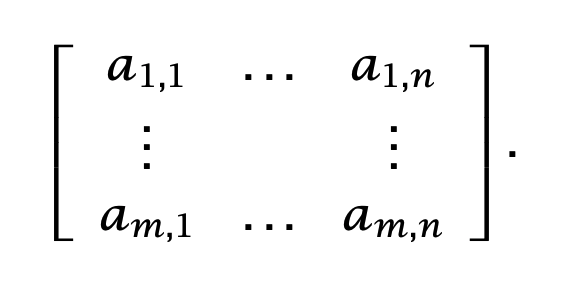
\includegraphics[width=.5\textwidth]{img/matrix.png}
    \end{figure}
    \item Use matrices to represent collections of data (each row is a vector)
    \item Matrices can represent images
\end{itemize}
\end{frame}

\begin{frame}
    \begin{figure}
    \centering
    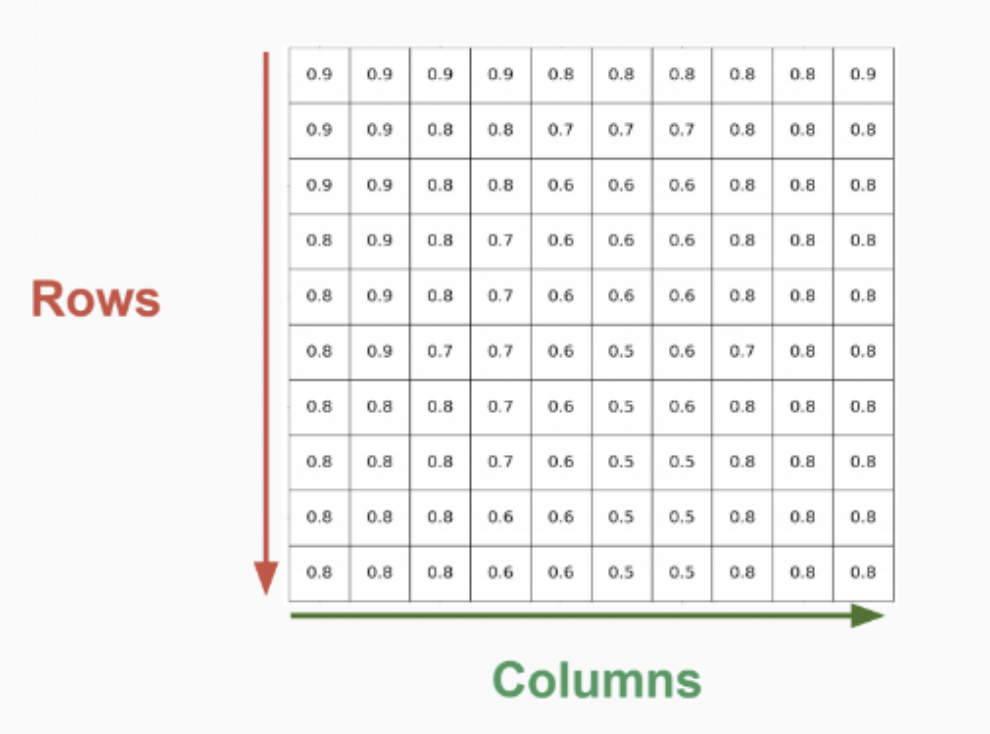
\includegraphics[width=.7\textwidth]{img/num_matrix.png}
    \caption{An example matrix filled with numbers}
    \end{figure}
\end{frame}